% CVPR 2023 Paper Template
% based on the CVPR template provided by Ming-Ming Cheng (https://github.com/MCG-NKU/CVPR_Template)
% modified and extended by Stefan Roth (stefan.roth@NOSPAMtu-darmstadt.de)

\documentclass[10pt,twocolumn,letterpaper]{article}

%%%%%%%%% PAPER TYPE  - PLEASE UPDATE FOR FINAL VERSION
% \usepackage[review]{cvpr}      % To produce the REVIEW version
% \usepackage{cvpr}              % To produce the CAMERA-READY version
\usepackage[pagenumbers]{cvpr} % To force page numbers, e.g. for an arXiv version

% Include other packages here, before hyperref.
\usepackage{graphicx}
\usepackage{amsmath}
\usepackage{amssymb}
\usepackage{booktabs}


% It is strongly recommended to use hyperref, especially for the review version.
% hyperref with option pagebackref eases the reviewers' job.
% Please disable hyperref *only* if you encounter grave issues, e.g. with the
% file validation for the camera-ready version.
%
% If you comment hyperref and then uncomment it, you should delete
% ReviewTempalte.aux before re-running LaTeX.
% (Or just hit 'q' on the first LaTeX run, let it finish, and you
%  should be clear).
\usepackage[pagebackref,breaklinks,colorlinks]{hyperref}


% Support for easy cross-referencing
\usepackage[capitalize]{cleveref}
\crefname{section}{Sec.}{Secs.}
\Crefname{section}{Section}{Sections}
\Crefname{table}{Table}{Tables}
\crefname{table}{Tab.}{Tabs.}


%%%%%%%%% PAPER ID  - PLEASE UPDATE
\def\cvprPaperID{*****} % *** Enter the CVPR Paper ID here
\def\confName{CVPR}
\def\confYear{2023}


\begin{document}

%%%%%%%%% TITLE - PLEASE UPDATE
    \title{Programing Assignement 1: Resnet}

    \author{Bingnan Li\\
    2020533092\\
    {\tt\small libn@shanghaitech.edu.cn}
    }
    \maketitle

%%%%%%%%% BODY TEXT


    \section{Resnet on CIFAR10}
    \label{sec:CIFAR10}

    In this section, I will introduce the implementation details and comparison between training from scratch and training with fine-tuning.
%-------------------------------------------------------------------------

    \subsection{Network Architecture}
    For this classification task, I use Resnet34 as the backbone and modified two layers to fit the input image size and the number of classes.
    The detailed modifications are as follows:
    \begin{itemize}
        \item Change the first convolution layer from $7\times 7$ kernel with stride 2 to $3\times 3$ kernel with stride 1.
        \item Change the final fully-connected layer from $1000$ output to $10$ output. 
    \end{itemize}

    \subsection{Global Training Settings}

    \subsubsection{Dataset split}
    \par The original CIFAR10 dataset contains 60000 images with size $32\times 32$ with 50000 for training and 10000 for testing.
    \par Given that it doesn't naturally split the validation set, I randomly choose 5000 images from the training set as the validation set with a fixed seed.

    \subsubsection{Data Augmentation}
    \par In order to increase the robustness and generalization of the model, I use random horizontal flip and random crop with zero padding as augmentation methods.

    \subsection{Training from scratch}

    \subsubsection{Training details}
    The hyperparameters settings follow the detail of~\cite{he2016deep}, which are listed as follows:
    \begin{itemize}
        \item learning rate: 0.1
        \item learning rate decay: decay 0.1 after 32k and 48k iterations.
        \item batch size: 128
    \end{itemize}
    Moreover, I used $Cross\ Entropy\ loss$ as loss function and used classification accuracy as metric

    \subsubsection{Experimental results}
    After 200 epoch training, the average classification accuracy is $\mathbf{91.31\%}$ under test set.
    The training curve are shown as Figure\ref{fig:train_curve}.
    \begin{center}
        \begin{figure}
            \includegraphics[width=0.5\textwidth]{images/CIFAR10_loss_curve}
            \caption{Training curve of Resnet34 on CIFAR10}
            \label{fig:train_curve}
        \end{figure}
    \end{center}

    \subsection{Training from Fine-tuning}
    Since I used $Resnet34$ as backbone, I can directly load the pretrained weight of $Resnet34$ trained on $ImageNet$.

    \subsubsection{Training Policy}
    Given that I only changed the first and the last of layer of $Resnet34$, I choose $semi$-$freezing$ $training$ policy to fine-tune.
    \par In detail, I freeze all the middle layers except the first and the last layer, and only train those two layers with learning rate 0.01
    for the first 50 epoch.
    Then I unfreeze all the layers and train the whole network with for the next 150 epoch.
    The learning rate decay changed to decay 0.1 after 10k and 35k iterations.

    \subsubsection{experimental results}
    After 200 epoch training, the average classification accuracy is $\mathbf{91.67\%}$ under test set.
    The training curve is shown as Figure\ref{fig:train_curve_finetune}.
    \begin{center}
        \begin{figure}
            \includegraphics[width=0.5\textwidth]{images/CIFAR10_ft_loss_curve}
            \caption{Training curve of Resnet34 on CIFAR10 with fine-tuning}
            \label{fig:train_curve_finetune}
        \end{figure}
    \end{center}
%-------------------------------------------------------------------------

    \subsection{Results Comparison and Analysis}
    I compared the accuracy and the epoch needed to converge\footnote{The epoch needed to converge is defined as the epoch after which the training loss doesn't decrese significantly.} between training from scratch and training with fine-tuning in Table~\ref{tab:cifar10_table}.
    \begin{table}
        \centering
        \caption{Comparison between different methods}
        \begin{tabular}{c c c}
            \hline
            method       & accuracy           & epoch to converge \\
            \hline
            from scratch & $91.31\%$          & $100$             \\
            fine-tuning  & $\mathbf{91.67\%}$ & $\mathbf{75}$     \\
            \hline
        \end{tabular}
        \label{tab:cifar10_table}
    \end{table}
    \par From the table, we can see that the accuracy of training with fine-tuning is slightly higher than training from scratch. Moreover, the training with fine-tuning converges faster than training from scratch.


    \section{Resnet on Crowd Counting}
    In this section, I explored the capability of $Resnet$ on Crowd Counting task.
    I used $Resnet18$ as backbone and choose $ShanghaiTech$ $Crowd$ $Counting$ $part$ $B$ dataset since it has the same
    image size and relative smaller number of heads.

    \subsection{Network Architecture}
    In this task, I followed the heatmap method proposed by~\cite{zhang2016single}, so the output of the network is a heatmap with the same size as the input image.
    To guarantee the output heatmap has the same size as the input image, I performed the following modifications:
    \begin{itemize}
        \item Removed the third and fourth residual block and added three to up-sampling blocks which contains has the architecture of Figure~\ref{fig:up_sample_block}.
        \item Removed the last fully-connected layer
    \end{itemize}
    The whole network architecture is shown as Figure~\ref{fig:CrowdCountingResnet}.
    \begin{center}
        \begin{figure}
            \includegraphics[width=0.5\textwidth]{images/Upsampling}
            \caption{Up-sampling block}
            \label{fig:up_sample_block}
        \end{figure}
    \end{center}
    \begin{center}
        \begin{figure}
            \includegraphics[width=0.5\textwidth]{images/CrowdCountingResnet}
            \caption{Network architecture of Resnet18 on Crowd Counting}
            \label{fig:CrowdCountingResnet}
        \end{figure}
    \end{center}

    \subsection{Training Settings}

    \subsubsection{Dataset split}
    \par The original ShanghaiTech dataset contains 716 images with size $768\times 1024$ with 400 for training and 316 for testing.
    I randomly choose 50 images from the training set as the validation set with a fixed seed.

    \subsubsection{Label preprocessing}
    \par The original label is a 2d vector which contains the coordinates of annotated head centers.
    In order to get the heat map from those labels, I followed the way of~\cite{zhang2016single} to generate the heat map using Gaussian kernel:
    \begin{equation}
        \label{eq:heat_map}
        F(\mathbf{x}) = \sum_{i=1}^N\delta (\mathbf{x-x_i})*G_{\sigma_i}(\mathbf{x})
    \end{equation}
    where $\sigma_i=\beta\times distance_{avg\_knn}$ is proportional to the average distance of the $k$ nearest neighbors of the $i$th point.
    Moreover, following~\cite{wang2019learning,gao2019c}, I dilated the intensity of heatmap by a factor of 100 so that
    the model will converge faster.

    \subsubsection{Loss function}
    Instead of using the loss function proposed by~\cite{zhang2016single}, I used $MSE$ loss as the loss function since I discovered that Zhang's loss function
    will cause extremly large loss value at the begining when the model is not pretrained from a good initialization.

    \subsection{Experimental results}
    Even though I used several tricks to boost training, the final result is still not as good as the result reported by~\cite{zhang2016single}.
    The comparison is shown in Table~\ref{tab:CrowdCountingResult}.
    \begin{table}
        \begin{center}
            \caption{Comparison between different methods}
            \begin{tabular}{c c c}
                \hline
                method                         & MAE              & MSE              \\
                \hline
                ours                           & $ 69.16$         & $ 103.51$        \\
                Zhang's~\cite{zhang2016single} & $ \mathbf{26.4}$ & $ \mathbf{41.3}$ \\
                \hline
            \end{tabular}\label{tab:CrowdCountingResult}
        \end{center}
    \end{table}

    \subsection{Analysis}
    \par I analyzed the middle layers of the network and found that the model pays more attention to the counter of different semantic regions
    instead of the heads. I assume there three reasons:
    \begin{itemize}
        \item Resnet18 is not deep enough to capture the fine-grained details of the heads because I visualized the predicted heatmap and discovered that the model pays more attention to
        the counter of different semantic regions instead of the heads.
        In Figure~\ref{fig:heatmap}, you can still see the counter of the bricks.
        \item The loss function does not constrain the spatial distribution of the predicted heatmap.
        \item Our output is a heatmap with the same size as the input image.
        However, in both~\cite{zhang2016single} and~\cite{wang2019learning}, the output size is downsampled, which may
        reduce the difficulty of the task.
    \end{itemize}
    \begin{center}
        \begin{figure}
            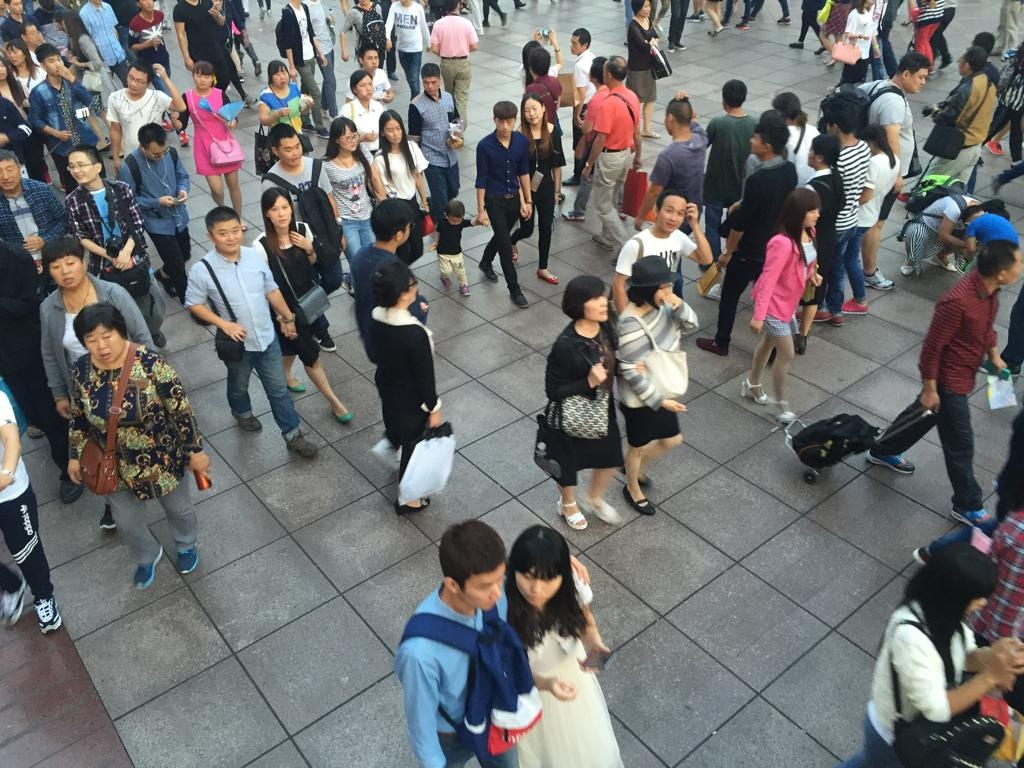
\includegraphics[width=0.15\textwidth]{images/input}
            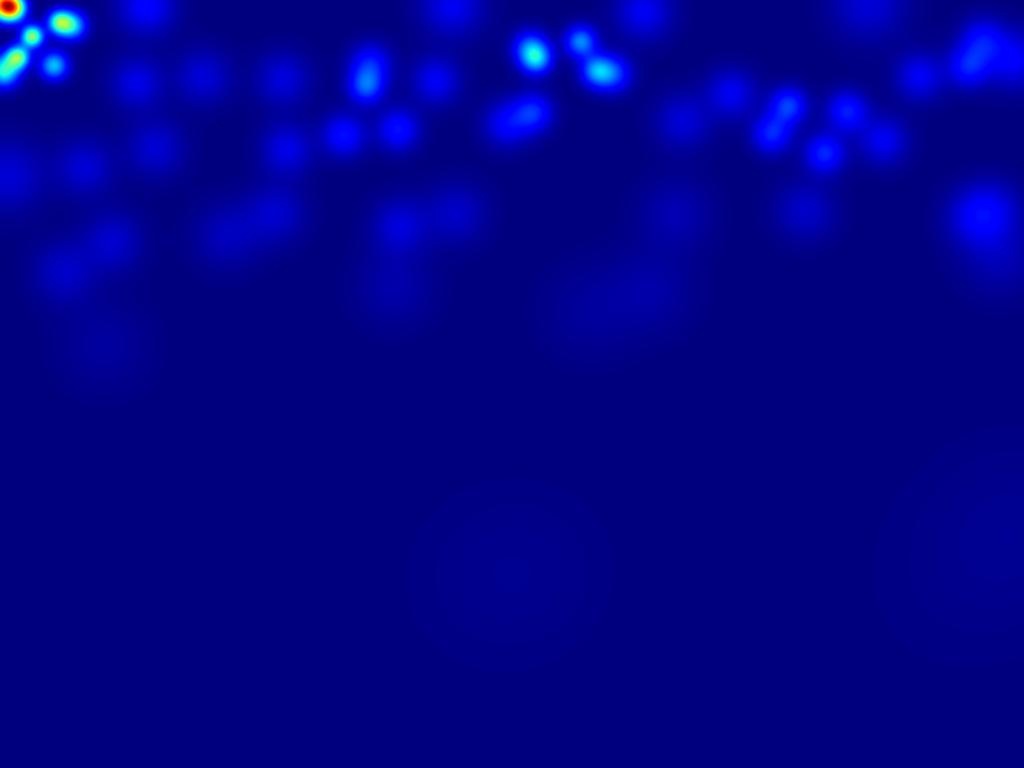
\includegraphics[width=0.15\textwidth]{images/gt}
            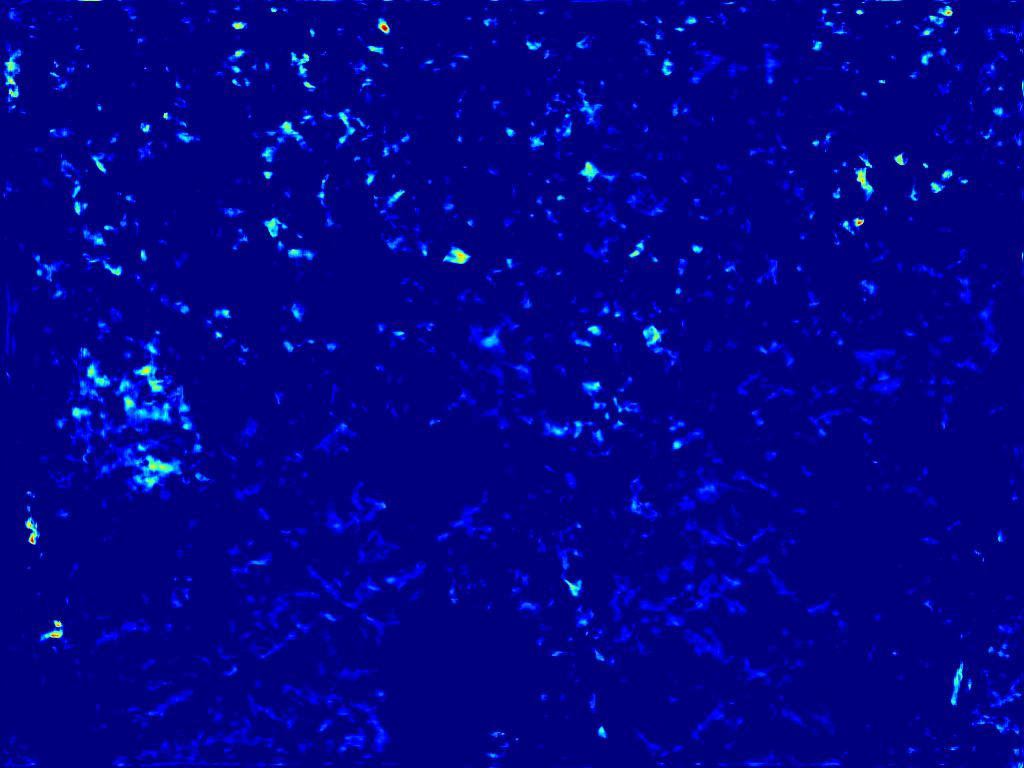
\includegraphics[width=0.15\textwidth]{images/pred_heat_map}
            \caption{Visualization of the input image, ground truth and predicted heatmap}
            \label{fig:heatmap}
        \end{figure}
    \end{center}



    {\small
    \bibliographystyle{ieee_fullname}
    \bibliography{egbib}
    }

\end{document}
